\section{Product Perspective}
	
This product is supposed to be part of an open source, under the GNU general Public License. It is a CAD software for programmers i.e. you code to make models. Customizer is the idea given by the user's only to fullfill their needs and It had been in demand even before it consentment. The Customizer will extent this already powerfull system by allowing user to design the genric models and modify the parameters without need to modify the program itself. It will also provide a way to modify the set of parameters using cmd-line.
	
The following are the main features that are included in OpenSCAD'customizer

\begin{enumerate}
	\item \textbf{Cross platform support:} Offers operating support for most of the known and commercial operating systems in form of binaries and also it can be compiled on other platforms.
	
	\item \textbf{Allows to modify parameters using GUI:} The system allows the user to easily modify the parameters of the given scad program using the GUI instead of changing it 
	manually.
	
	\item \textbf{Backward Compatibilty:} OpenSCAD should be backward compatibilty even after new features are implemented.
	
	\item \textbf{Easy to use syntax:} The syntax for creating the input widget, groups and description in customzier. Should be easy to use.
	
	\item \textbf{Abiltiy to manage parameters:} It should be easy to manage the parameters by grouping them or giving them option to hide or unhide them.
	
	\item \textbf{Feature to save different set of parameters:} Feature to save different set of parameters with customized name should be provided. So, that given set could be used in future.
	
	\item \textbf{Feature to modify saved sets:} User should be able to modify,delete the already saved ets of parameters.
	
\end{enumerate}	

\section{product functions}

Functions performed by Customizer are:
\begin{itemize}
	\item {\bf Provides Syntax to generate widget to modify parameter}: This means there is a syntax which could be used to generate different widget for different type of pararmeters.
	The widgets that we entend to support are: 
	\begin{enumerate} 
		\item Spinbox:
		\begin{enumerate}
			\item With Increment Size
			\item without Increment Size 
		\end{enumerate} 
		\item Checkbox 
		\item Slider
		\begin{enumerate}
			\item with Increment Size
			\item With Default Increment Size
		\end{enumerate}
		\item Textbox
		\item Special vector 
		\item Combo Box
		\begin{enumerate}
			\item Simple
			\item Labeled 
		\end{enumerate}
		
		\begin{table}[h]
			\centering
			\begin{tabular}{ |c|c|c|c|c|c| }
				\hline
				& \multicolumn{5}{|c|}{Type of Widgets} \\
				\hline
				Type of Data&	Number&	String&	BOOL &Vector &Range	 \\ [0.5ex]
				\hline 
				SpinBox&Y&	-&	-&	-&	- \\ \hline
				ComboBox&	Y&	Y&	-&	-&	- \\ \hline
				Text&	Y&	Y&	-&	Y&	- \\ \hline
				Slider&	Y&	-&	-&	-&	- \\ \hline
				VectorWidget&	-&	-&	-&	Y&- \\ \hline
				Checkbox&	-&	-&	Y&	-&	- \\ [1ex]
				\hline
			\end{tabular}
			\caption{Table to show the support of widgets for different DataType}
			\label{table2}
		\end{table}
		
	\end{enumerate}
	
	\item \textbf{Provide Syntax for attribute of parameter widget to be created:} 
	Customzier also provide syntax to provide aditional attribute of the parameter
	
	\begin{table}[h]
		\centering
		\begin{tabular}{ |c|c|c|c|c|c|c| }
			\hline
			& \multicolumn{6}{|c|}{Type of Widgets} \\
			\hline
			&Max&	Min &	List of items&	Step size&	Label List	 &Default	 \\ [0.5ex]
			\hline 
			SpinBox& -&	-&	-&	Y&	 -& Y \\ \hline
			ComboBox&	-&	-&	Y&	-&	Y&Y \\ \hline
			Text&	-&	-&	-&	-&	-&Y \\ \hline
			Slider&	Y&	Y&	-&	Y&	-&Y \\ \hline
			Vector&	-&	-&	-&	-&	-&Y \\ \hline
			Checkbox&	-&	-&	-&	-&	-&Y \\ [1ex]
			\hline
		\end{tabular}
		\caption{Table to show the support of attributes  for different widgets}
		\label{table2}
	\end{table}
	
	\item {\bf Provides Syntax to Describe parameter}: 
	This means there is a syntax which could be used to provide description for the parameter.
	
	\item \textbf{Provides Syntax to Group Parameter}:
	This means there is a syntax which could be used to group the parameters into different groups or tab to easily manage Customizer and make customizer interface little simple.
	
	\item \textbf{Provides Syntax to Hide parameters}
	This means there is a syntax which could be used to Hide certain parameters.
	
	\item \textbf{Provides Syntax to make certain parameters Global}
	This means there is a syntax which could be used to make certain parameters gloabal i.e. they are present in each and every group.

	\item \textbf{Provides option to reset parameters:}
	All parameters in customizer could be reset to default value just by the click of a button.

	\item \textbf{Provides option to Hide description:}
	Description of all the parameters in customizer could be Hidden value just by the click of a button.
	
	\item \textbf{Provides Save the set of parameters in JSON file}:
	This feature provides a way that give user the ability to save the value of the parameter and also we can apply them through the cmd-line and get the output.
	
	\item \textbf{Provides GUI to add Set of Parameters}
	This means there is a way to store different set of parameters which represent different models from generic model.
	
	\item \textbf{Provides Cmd-line support to apply Set of Parameters:}
	This means that values of parameter for given set can be applied to model using the cmd-line argument.
	
	 
\end{itemize}

\section{User Characteristics}

We have identified five potential classifications of users of our system: 

\begin{enumerate}
	\item Desingers: Desingers are the people how code to create model their for their own use or for comercial use.
	\item The Client: These are the people which will customzie model to their need made by modellers before ordering or printing model themselves. 
	\item Developers: These are people who might want to integrate this new feature of OpenSCAD into their systems.
	
\end{enumerate}

\subsection{The General User}

All users can be assumed to have the following characteristics:

\begin{enumerate}
	\item Ability to read and understand English.
	\item Familiarity with the operation of the basic Graphical User Interface (GUI) components of OpenSCAD.
	\item Beyond the above, no further facility with computer technology can be assumed.
\end{enumerate}

\subsection{Designers:}
The Designer users can be assumed to have the following characteristics:
\begin{enumerate}
	\item Basic Knowledge of OpenSCAD.
	\item Basic Knowledge of Creating models.
	\item Basic coding skills.
	\item Optional experience of cmd-line.
\end{enumerate}

\subsection{Developers:}
The Designer users can be assumed to have the following characteristics:
\begin{enumerate}
	\item Basic Knowledge of programming.
	\item Knowledge of JSON.
	\item Ability to program in cmd-line.
\end{enumerate}




\section{DFDs}
A data flow diagram (DFD) is a graphical representation of the "flow" of data through an information system, modeling its process aspects. A DFD is often used as a preliminary step to create an overview of the system, which can later be elaborated. DFDs of DoS is as following-:
\begin{enumerate}
\item Data flow LEVEL 0 figure \ref{fig:DFDs}
\item Data flow LEVEL 1 figure \ref{fig:DFDs1}
\end{enumerate}

\begin{figure}[H]
\centering
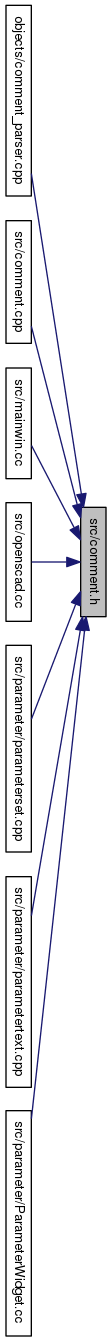
\includegraphics[width=0.7\linewidth]{images/comment}
\caption{}
\label{fig:comment}
\end{figure}
\begin{figure}[H]
\centering
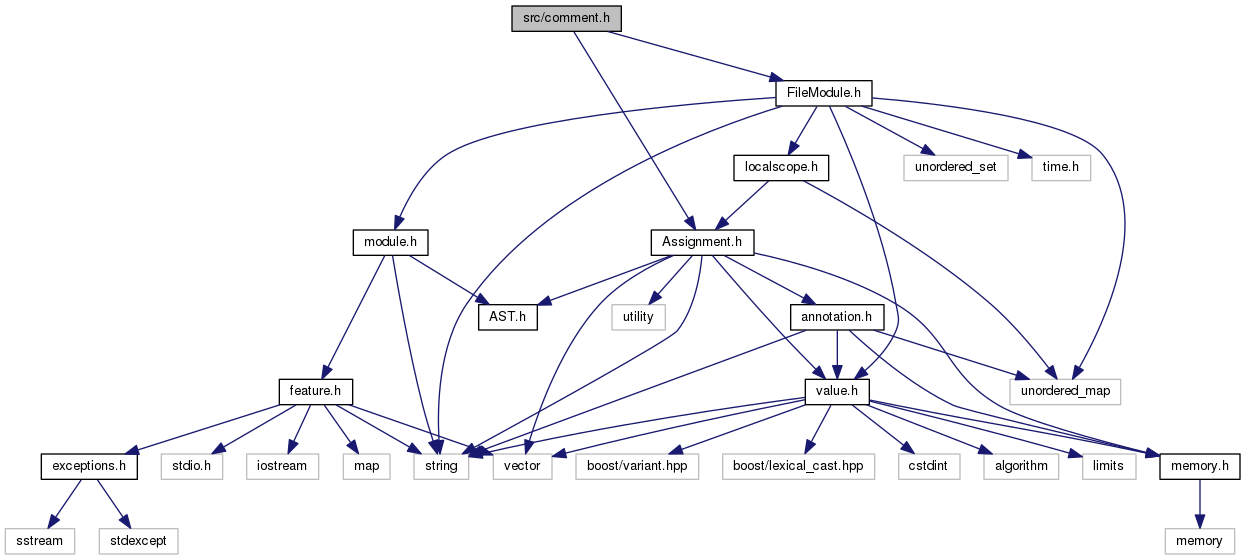
\includegraphics[width=0.7\linewidth]{images/comment1}
\caption{}
\label{fig:comment1}
\end{figure}

Here, In figure \ref{fig:DFDs} and figure \ref{fig:DFDs1}
\begin{enumerate}
\item MSG means Message
\item initial represent all initial input value
\item matrix represent all Mass, Height, Stiffness matrix
\end{enumerate}

\section{Flowchart}
A flowchart is a type of diagram that represents an algorithm, work flow or process, showing the steps as boxes of various kinds, and their order by connecting them with arrows
and following is the flowchart of customizer showing flow of control and Data in the software-:

\begin{figure}
	\centering 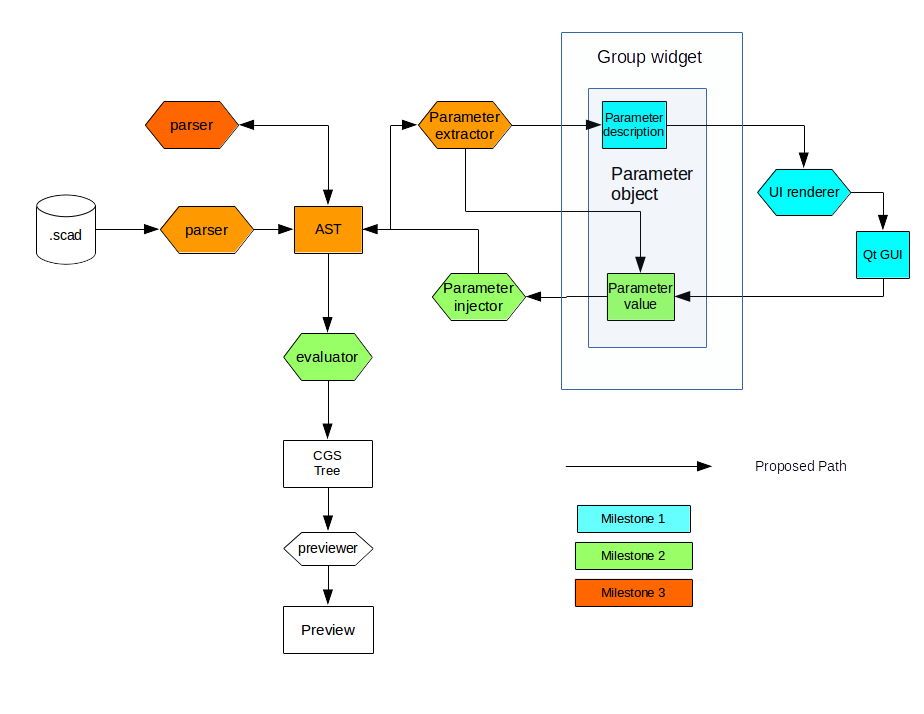
\includegraphics[scale=0.6]{images/flowchart.png}
	\caption{Flowchart of Customizer}
	\label{fig:FD1}
\end{figure}

\subsection{Detailed Description}

The basic implementation of the this project is almost done in form of prototype. There is need to modify structure of the project. We have to divide the task in to there parts:

\begin{enumerate}
	\item \textbf{Front end}
	It will deal with how the parameter will look to user like in form of range or spinbox etc. This part will include two parts:
	\begin{enumerate}
		\item \textbf{Individual Parameter}
		This will define how individual parameters will look like
		\item \textbf{Container Widget}
		This will contain UI features common to all parameter. This widget will contain all parameter widget. 
		
	\end{enumerate}
	
	\item \textbf{Back End}
	This will include the parser part that will create AST nodes and we can extract the parameters from the AST. we can use the single parser for whole .scad file or separate parser for extracting the parameters with annotations.
	
	The Back end part will also include the parameter extractor and injector or the injector can be included in parameter object which will serve as interface 
	\item \textbf{Interface}
	This will include the parameter object which will serve as interface between both Back end and Front end. Parameter object will contain information regarding each individual parameter like parameter name, default value and information how these parameter will be displayed as widgets to user. Parameter object could also include the method to inject the value of individual parameter in to the AST. 
	
\end{enumerate}

\section{Class Diagrams}
\begin{figure}[H]
	\centering
	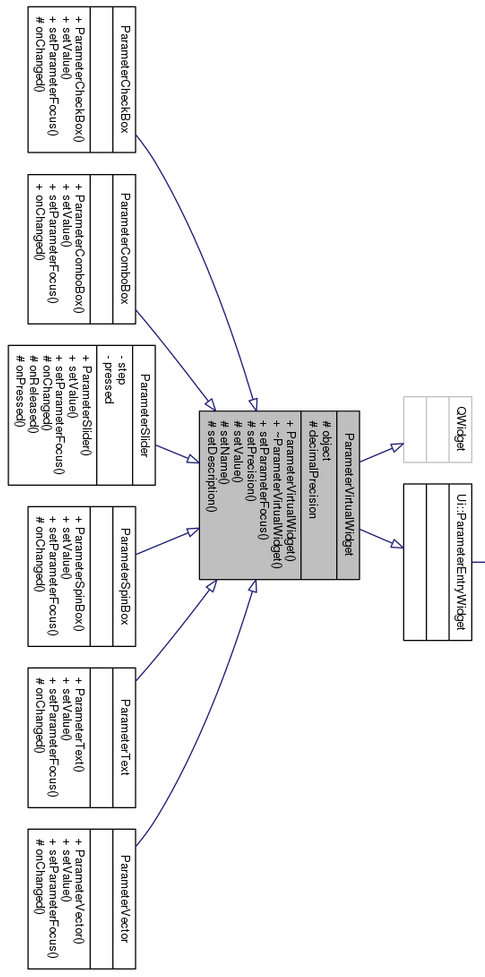
\includegraphics[width=1\linewidth]{images/collaborative1}
	\caption{Class Diagram for Customizer (Part A) }
	\label{fig:collaborative1}
\end{figure}
\begin{figure}[H]
	\centering
	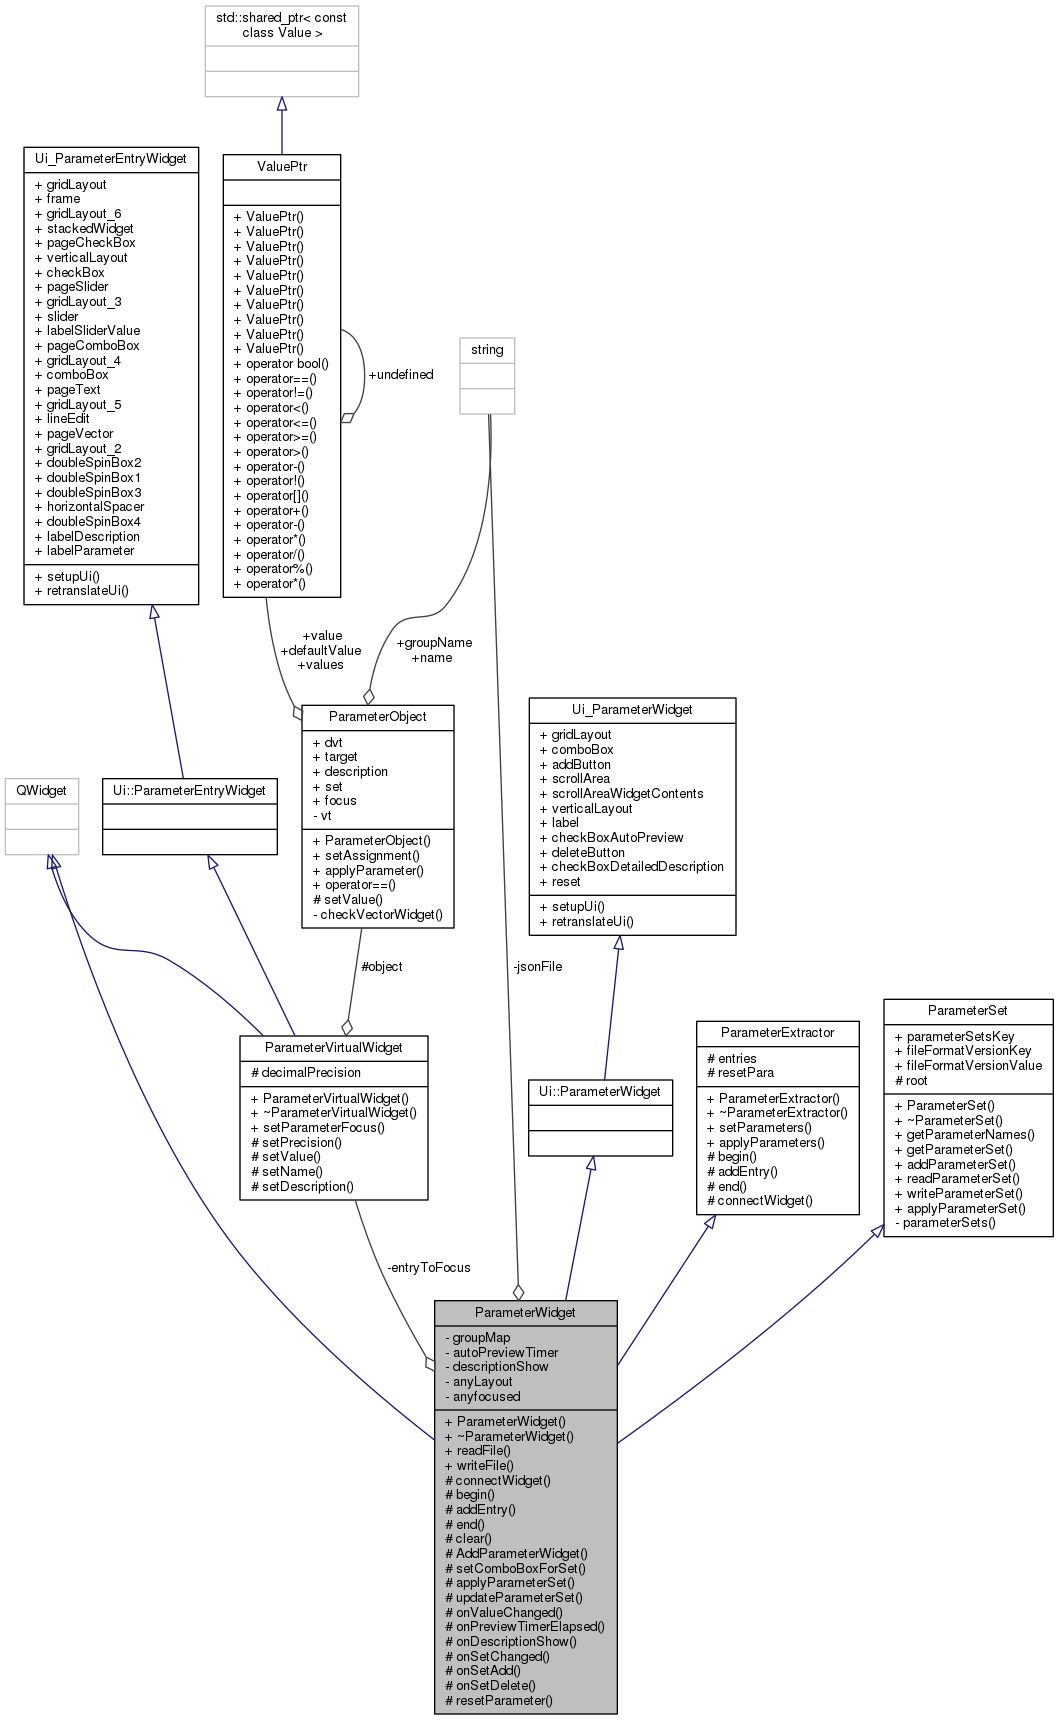
\includegraphics[scale=0.40]{images/collaborative}
	\caption{Class Diagram for Customizer (Part B)}
	\label{fig:collaborative}
\end{figure}
